\documentclass[11pt]{article}

\usepackage[margin=1in]{geometry}
\usepackage{kotex}
\usepackage{amsmath,amssymb,amsthm}
\usepackage{booktabs}
\usepackage{graphicx}
\usepackage{enumitem}
\usepackage[numbers,sort&compress]{natbib}
\usepackage[colorlinks=true,allcolors=blue]{hyperref}

\theoremstyle{definition}
\newtheorem{proposition}{명제}
\newtheorem{assumption}{가정}
\renewcommand{\proofname}{증명}
\renewcommand{\abstractname}{초록}
\renewcommand{\figurename}{그림}
\renewcommand{\tablename}{표}
\renewcommand{\refname}{참고문헌}

\title{HydraLoRA를 결합한 Foveated Local Loops:\\
VRAM 제약형 비전 월드모델의 국소 증거 획득 구조}

\author{저자 정보 생략: 학회 공유용 초안}
\date{2026년 5월 3일}

\begin{document}
\maketitle

\begin{abstract}
비전 월드모델은 보통 장면을 압축된 latent state로 표현하고 다음 상태를 예측하는 모델로 설명된다.
그러나 실제 시각 추론에서는 전체 장면만큼이나 작은 국소 증거가 중요하다.
예를 들어 회로도나 PCB 이미지에서는 핀 번호, 배선 접점, 극성 표식, 미세 결함 하나가 전체 그래프 해석을 바꿀 수 있다.
모든 픽셀을 균일한 고해상도로 처리하면 visual token, activation, KV cache 비용이 급격히 커지고, 반대로 crop만 보면 국소 증거의 의미를 결정하는 전역 문맥이 사라진다.
본 초안은 저해상도 전역 루프와 고해상도 국소 루프를 분리하는 foveated vision world model 구조를 제안한다.
전역 루프는 predictive latent state, coarse topology, uncertainty, task context를 유지하고, 국소 루프는 소수의 ROI(region of interest)를 고해상도로 재관찰하여 typed evidence를 추출한 뒤 graph-like memory를 갱신한다.
국소 시각 skill을 효율적으로 쓰기 위해 Simula 방식으로 학습된 Local LoRA Bank를 HydraLoRA식 shared-$A$/multi-$B$ expert 구조로 재조직하고, runtime에서는 certified bundle만 선택한다.
또한 token-aware VRAM budget, adapter parameter saving, top-$k$ expert routing, residual-driven synthetic curriculum, graph-memory update를 수식으로 정리한다.
\end{abstract}

\section{서론}

이 연구의 출발점은 단순하다.
비전 월드모델이 전체 장면을 계속 기억하면서도, 비싼 고해상도 계산은 정말 필요한 곳에만 쓸 수 있을까?
이 질문은 회로도와 PCB 이미지에서 특히 선명해진다.
저해상도 이미지는 전체 배치와 큰 연결 구조를 보존하지만, 작은 글자, 접점, 극성, 납땜 결함 같은 정보는 쉽게 지워진다.
반대로 전체 이미지를 고해상도로 넣으면 visual token 수, activation memory, key-value(KV) cache가 커져 제한된 VRAM 환경에서는 부담이 크다.
또한 crop만 보는 단순 파이프라인은 싸지만, 그 crop이 왜 중요한지, 그 증거가 전체 graph state를 어떻게 바꾸는지 설명하기 어렵다.

본 초안은 ``HydraLoRA를 결합한 Foveated Local Loops''를 제안한다.
구조는 크게 저해상도 global loop, high-recall ROI proposal, 고해상도 local loop, HydraLoRA 기반 local-skill router, typed evidence extractor, graph-memory update loop로 나뉜다.
전체 방향은 world model과 JEPA 계열 latent prediction \citep{ha2018worldmodels,hafner2023dreamerv3,assran2023ijepa,bardes2024vjepa,maes2026leworldmodel}, LoRA/QLoRA 기반 parameter-efficient adaptation \citep{hu2021lora,dettmers2023qlora}, HydraLoRA \citep{tian2024hydralora}, Simula의 reasoning-driven synthetic data generation \citep{davidson2026simula}에서 근거를 얻는다.

이 글은 완성된 실험 논문이 아니라, 학회 내부 공유와 피드백을 위한 수학적으로 정리된 연구 제안서에 가깝다.
핵심 기여는 다음 다섯 가지다.
\begin{enumerate}[leftmargin=*]
  \item global state, ROI crop, typed evidence, graph memory를 포함하는 foveated observation model을 정의한다.
  \item adapter memory와 visual token/KV cache 비용을 분리한 VRAM budget을 제시한다.
  \item 독립 LoRA bank와 shared-$A$ HydraLoRA bank의 parameter saving을 명제로 정리한다.
  \item 월드모델의 prediction residual을 Simula-style local training data로 되돌리는 curriculum 식을 제안한다.
  \item 회로도/PCB 도메인을 대상으로 한 실험군, 지표, ablation protocol을 제시한다.
\end{enumerate}

\begin{figure}[t]
  \centering
  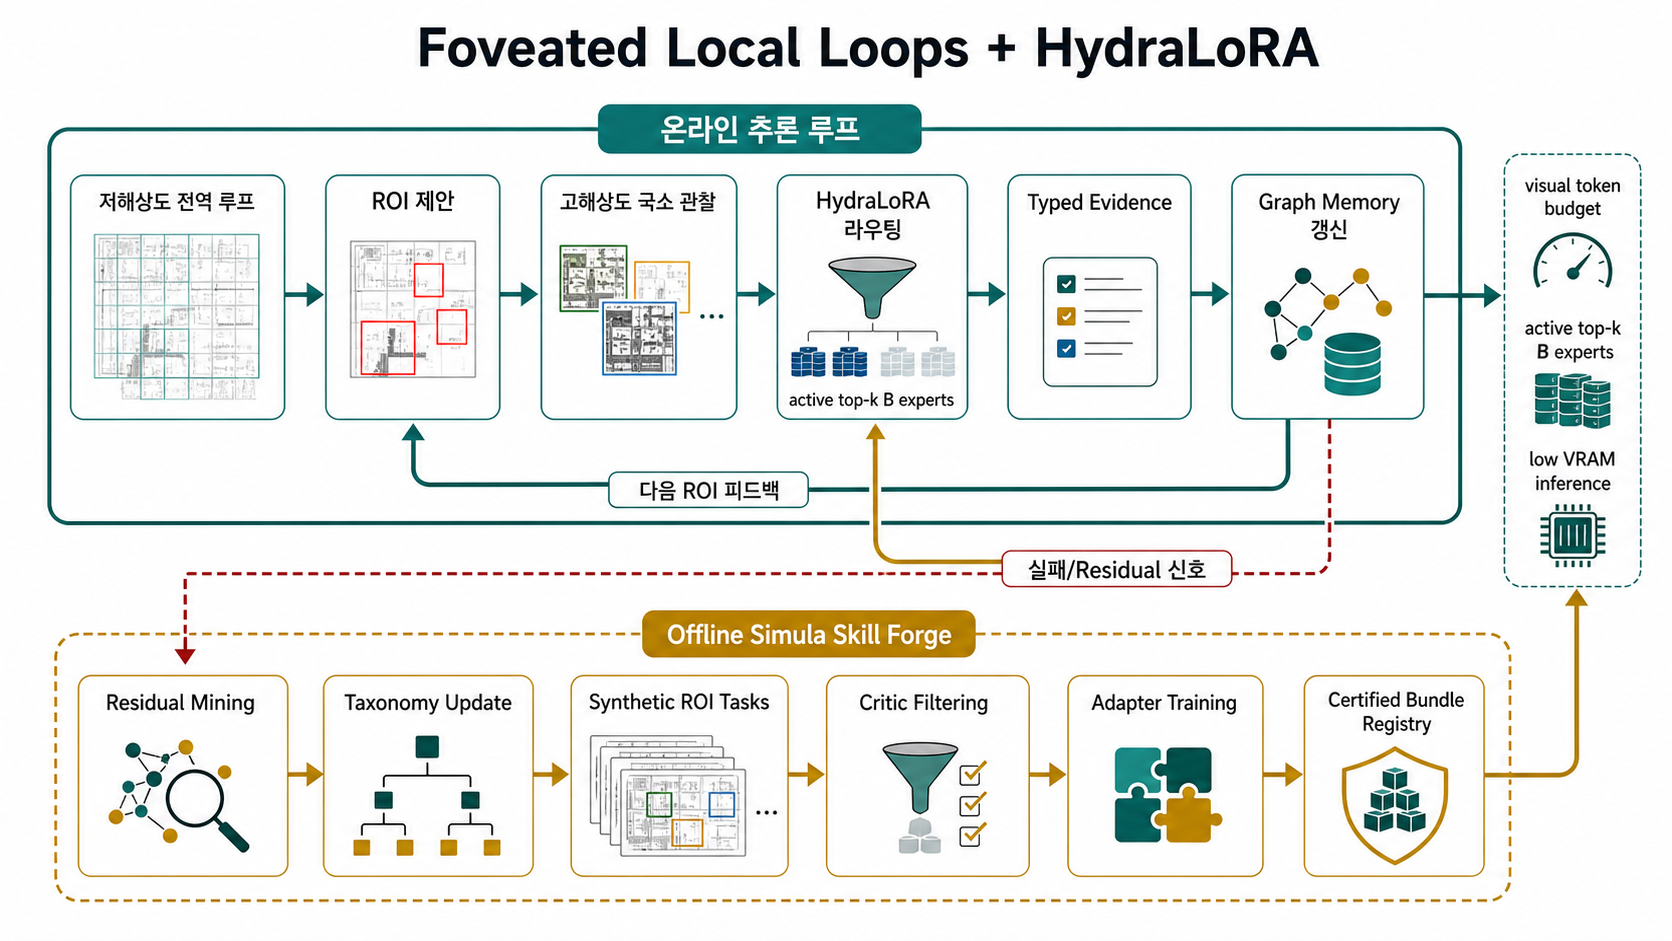
\includegraphics[width=\linewidth]{figures/foveated_hydralora_loop_imagegen.png}
  \caption{제안하는 foveated loop의 요약. 전역 루프는 저해상도 상태를 유지하고, 국소 루프는 필요한 ROI만 고해상도로 보며, 추출된 증거는 다시 graph memory와 다음 ROI 선택에 반영된다. Offline Simula Skill Forge는 residual을 받아 local skill adapter와 certified bundle registry를 갱신한다.}
  \label{fig:foveated-loop-ko}
\end{figure}

\section{관련 연구}

\paragraph{월드모델과 latent prediction.}
World model은 장면이나 환경의 내부 동역학을 압축적으로 학습하여 perception, planning, control에 쓰려는 접근이다 \citep{ha2018worldmodels,hafner2023dreamerv3}.
JEPA 계열 방법은 pixel reconstruction 대신 representation space에서 예측을 수행한다 \citep{assran2023ijepa,bardes2024vjepa}.
LeWorldModel(LeWM)은 raw pixel에서 안정적으로 학습되는 JEPA-style latent world model을 제안했다는 점에서 본 연구의 전역 루프 설계에 중요한 참고점이다 \citep{maes2026leworldmodel}.
다만 본 초안의 목표는 action-conditioned control 자체가 아니라, 정적 또는 준정적 시각 자료에서 국소 증거를 획득하고 memory를 갱신하는 perception layer다.

\paragraph{LoRA bank와 HydraLoRA.}
LoRA는 base weight $W_0$를 freeze하고 low-rank update $\Delta W=BA$만 학습하는 방식이다 \citep{hu2021lora}.
QLoRA는 quantized base model과 LoRA를 결합해 제한된 GPU memory에서도 fine-tuning을 가능하게 한다 \citep{dettmers2023qlora}.
그러나 skill 수가 늘어나면 ``LoRA 하나가 작다''는 사실만으로는 충분하지 않다.
adapter weight, GPU resident memory, adapter loading, routing, bundle compatibility 비용이 누적되기 때문이다.
HydraLoRA는 여러 LoRA의 $A$ matrix는 공유성이 크고 $B$ matrix는 task/domain 차이를 더 잘 담는다는 관찰에 기반하여 shared-$A$/multi-$B$ 구조를 제안한다 \citep{tian2024hydralora}.
본 연구는 이를 국소 시각 skill bank의 조직 원리로 재해석한다.

\paragraph{Simula와 synthetic curriculum.}
Simula는 synthetic data generation을 단순 데이터 증식이 아니라 taxonomy, global/local diversification, complexification, critic filtering으로 제어하는 mechanism design 문제로 본다 \citep{davidson2026simula}.
본 초안에서 Simula는 runtime 추론기가 아니라 offline skill forge다.
즉, 실패 로그, graph conflict, uncertain ROI case를 받아 local adapter와 router를 학습시키는 데이터로 바꾸는 계층이다.

\section{문제 정의}

$I_t \in \mathbb{R}^{H \times W \times 3}$를 시점 또는 inspection step $t$에서의 이미지라고 하자.
정적 회로/PCB 분석에서는 $t$가 실제 시간이라기보다 반복 관찰 단계일 수 있다.
시스템은 global latent state $z_t \in \mathbb{R}^{d_z}$, graph memory $G_t=(V_t,E_t,\psi_t)$, evidence table $\mathcal{E}_t$를 유지한다.
$\psi_t$는 component label, pin connection, junction state, polarity, defect annotation 같은 graph attribute에 대한 belief를 저장한다.

\paragraph{Foveated observation.}
전역 루프는 저해상도 이미지
\begin{equation}
  x_t^g = D_\rho(I_t)
\end{equation}
를 관측한다.
여기서 $D_\rho$는 downsampling 연산이다.
ROI 루프는 최대 $K$개의 box를 선택한다.
\begin{equation}
  \mathcal{R}_t = \{r_{t,1},\ldots,r_{t,k_t}\}, \qquad k_t \le K.
\end{equation}
각 ROI에 대해서는 margin $m_j$를 포함한 고해상도 crop을 만든다.
\begin{equation}
  x_{t,j}^{\ell} = C(I_t,r_{t,j},m_j).
\end{equation}
따라서 전체 관측은 다음처럼 쓸 수 있다.
\begin{equation}
  o_t = \left(x_t^g,\{x_{t,j}^{\ell}\}_{j=1}^{k_t},G_t,\mathcal{E}_t\right).
\end{equation}

\paragraph{전역 latent prediction.}
전역 encoder $E_g$와 predictor $P$는
\begin{equation}
  z_t = E_g(x_t^g,G_t), \qquad
  \hat z_{t+1}=P(z_t,u_t)
\end{equation}
를 정의한다.
$u_t$는 현재 query, inspection action, task context를 뜻한다.
LeWM-style 관점에서 전역 루프의 학습 objective는 latent prediction loss와 anti-collapse regularizer를 포함할 수 있다.
\begin{equation}
  \mathcal{L}_{\mathrm{global}}
  =
  \left\|\hat z_{t+1} - \mathrm{sg}(z_{t+1})\right\|_2^2
  +
  \lambda_{\mathrm{sig}}\mathcal{D}_{\mathrm{sig}}(\{z_t\},\mathcal{N}(0,I)).
  \label{eq:global-loss-ko}
\end{equation}
$\mathrm{sg}$는 stop-gradient를 뜻한다.
$\mathcal{D}_{\mathrm{sig}}$는 latent sample들의 random one-dimensional projection이 표준정규분포와 얼마나 다른지 측정하는 regularizer로 볼 수 있다.
이 초안에서는 LeWM의 정확한 regularizer를 재증명하지 않고, collapse를 막고 compact predictive state를 유지하는 역할에 초점을 둔다.

\paragraph{Residual을 local data signal로 쓰기.}
Prediction residual은 단순 scalar loss가 아니다.
본 초안에서는 다음처럼 구조화된 residual을 둔다.
\begin{equation}
  \delta_t =
  \left[
  d_z(\hat z_{t+1},z_{t+1}),
  d_G(\hat G_{t+1},G_{t+1}),
  1-\bar c_t,
  \chi_{\mathrm{conflict}}(G_t,\mathcal{E}_t)
  \right].
  \label{eq:residual-ko}
\end{equation}
$d_z$는 latent mismatch, $d_G$는 graph inconsistency, $\bar c_t$는 evidence confidence 평균, $\chi_{\mathrm{conflict}}$는 상충하는 local claim이 있는지를 나타낸다.
Offline Simula loop는 이 residual을 taxonomy node, hard negative, ROI label, required local skill로 변환한다.

\section{방법}

\subsection{Budget-aware ROI selection}

$T_g$를 저해상도 전역 이미지의 visual token 수, $T_j$를 ROI crop $j$의 token 수라고 하자.
Patch size가 $p$이고 crop 크기가 $h_j\times w_j$이면
\begin{equation}
  T_j \approx \left\lceil \frac{h_j}{p} \right\rceil
          \left\lceil \frac{w_j}{p} \right\rceil.
\end{equation}
전체 visual token 수는
\begin{equation}
  T_{\mathrm{vis}} = T_g + \sum_{j=1}^{k_t} T_j.
  \label{eq:tokens-ko}
\end{equation}

ROI scheduler는 각 후보 $r$에 다음 utility를 부여한다.
\begin{equation}
  U(r)
  =
  \alpha u_{\mathrm{unc}}(r)
  + \beta u_{\mathrm{task}}(r)
  + \gamma u_{\mathrm{graph}}(r)
  + \xi u_{\mathrm{failure}}(r)
  - \eta c_{\mathrm{tok}}(r)
  - \mu c_{\mathrm{adapt}}(r).
  \label{eq:roi-utility-ko}
\end{equation}
앞의 네 항은 uncertainty, task relevance, graph conflict, historical failure를 반영하고, 뒤의 두 항은 token cost와 adapter cost를 반영한다.
선택 문제는 작은 budgeted selection 문제로 쓸 수 있다.
\begin{equation}
  \mathcal{R}_t^\star
  =
  \arg\max_{\mathcal{R}\subseteq \mathcal{C}_t}
  \sum_{r\in\mathcal{R}} U(r)
  \quad
  \mathrm{s.t.}
  \quad
  |\mathcal{R}|\le K,\quad
  T_g+\sum_{r\in\mathcal{R}}T(r)\le T_{\max}.
  \label{eq:roi-select-ko}
\end{equation}
$\mathcal{C}_t$는 high-recall ROI candidate set이다.
초기 MVP에서는 orchestration spec에 맞춰 $K=3$을 기본값으로 둔다.

\subsection{VRAM accounting}

Peak memory는 다음처럼 근사할 수 있다.
\begin{equation}
  M_{\mathrm{peak}}
  \approx
  M_{\mathrm{base}}(q)
  + M_{\mathrm{adapt}}(\mathcal{B}_t)
  + M_{\mathrm{KV}}(T_{\mathrm{vis}})
  + M_{\mathrm{act}}(B,T_{\mathrm{vis}})
  + M_{\mathrm{misc}}.
  \label{eq:vram-ko}
\end{equation}
$q$는 base model precision, $\mathcal{B}_t$는 active certified adapter bundle, $B$는 batch size다.
$M_{\mathrm{misc}}$에는 runtime allocator overhead 등이 포함된다.
Layer 수가 $L$, hidden dimension이 $d$, KV precision이 $b_{\mathrm{kv}}$ bytes이면 KV cache는 간단히
\begin{equation}
  M_{\mathrm{KV}}(T_{\mathrm{vis}})
  \approx
  2 L B T_{\mathrm{vis}} d\, b_{\mathrm{kv}}
  \label{eq:kv-ko}
\end{equation}
로 볼 수 있다.
이 식은 왜 LoRA weight만 줄이는 것이 부족한지 보여준다.
고해상도 ROI 수와 visual token 수를 함께 관리하지 않으면 peak VRAM은 여전히 커질 수 있다.

\begin{proposition}[Foveated token ratio]
원본 이미지 $H\times W$를 전체 고해상도로 처리할 때 token 수를 $T_{\mathrm{full}}\approx HW/p^2$라고 하자.
Foveated system이 $H_g\times W_g$ 크기의 global image와 $h\times w$ 크기의 ROI crop $K$개를 쓴다면,
\begin{equation}
  \frac{T_{\mathrm{fov}}}{T_{\mathrm{full}}}
  \approx
  \frac{H_gW_g + Khw}{HW}.
  \label{eq:fov-ratio-ko}
\end{equation}
\end{proposition}

\noindent\textbf{증명.}
같은 patch size $p$를 쓴다고 하면, global token 수는 $H_gW_g/p^2$, 각 crop token 수는 $hw/p^2$이다.
따라서 $T_{\mathrm{fov}}\approx (H_gW_g+Khw)/p^2$이고, 이를 $T_{\mathrm{full}}\approx HW/p^2$로 나누면 식 \ref{eq:fov-ratio-ko}가 나온다. \hfill$\square$

\subsection{HydraLoRA local skill bank}

Frozen linear layer $W_0\in\mathbb{R}^{d_{\mathrm{out}}\times d_{\mathrm{in}}}$에 대해 독립 LoRA expert $i$는
\begin{equation}
  W_i = W_0 + \frac{\alpha}{r}B_iA_i,
  \qquad
  A_i\in\mathbb{R}^{r\times d_{\mathrm{in}}},
  \quad
  B_i\in\mathbb{R}^{d_{\mathrm{out}}\times r}
\end{equation}
를 사용한다.
HydraLoRA는 $A$를 공유하고 skill-specific $B_i$를 여러 개 둔다.
\begin{equation}
  W(x)=W_0+\frac{\alpha}{r}\sum_{i\in S_k(x)}g_i(x)B_iA.
  \label{eq:hydra-ko}
\end{equation}
$g_i(x)$는 router score이고 $S_k(x)$는 top-$k$ expert set이다.
Router input은 global context, ROI embedding, ROI type hint, task instruction, complexity estimate, registry metadata를 결합한다.
\begin{equation}
  g(x)=\mathrm{softmax}\left(R_\phi([z_t,h_j,\tau_j,q_t,c_j])\right).
\end{equation}

\begin{proposition}[Adapter parameter saving]
하나의 adapted layer에서 expert 수가 $N$, rank가 $r$일 때 독립 LoRA bank의 parameter 수는
\begin{equation}
  P_{\mathrm{bank}} = N r(d_{\mathrm{in}}+d_{\mathrm{out}})
\end{equation}
이고, shared-$A$ HydraLoRA bank의 parameter 수는
\begin{equation}
  P_{\mathrm{hydra}} = r d_{\mathrm{in}} + N r d_{\mathrm{out}}.
\end{equation}
$d_{\mathrm{in}}=d_{\mathrm{out}}=d$이면
\begin{equation}
  \frac{P_{\mathrm{hydra}}}{P_{\mathrm{bank}}}=\frac{N+1}{2N}.
  \label{eq:hydra-ratio-ko}
\end{equation}
또한 $N$개 중 $k$개의 $B$ expert만 GPU에 올린다면, 전체 독립 bank를 GPU에 상주시킨 경우 대비 active adapter parameter ratio는
\begin{equation}
  \frac{P_{\mathrm{active}}}{P_{\mathrm{bank}}}=\frac{k+1}{2N}
  \label{eq:active-ratio-ko}
\end{equation}
이다.
\end{proposition}

\noindent\textbf{증명.}
독립 bank는 $A_i$와 $B_i$를 expert마다 하나씩 저장하므로 $Nr d_{\mathrm{in}}+Nr d_{\mathrm{out}}$개의 parameter를 가진다.
Hydra bank는 $A$ 하나와 $N$개의 $B_i$를 저장하므로 $rd_{\mathrm{in}}+Nr d_{\mathrm{out}}$개다.
Square layer 조건 $d_{\mathrm{in}}=d_{\mathrm{out}}=d$를 대입하면 식 \ref{eq:hydra-ratio-ko}가 나온다.
Top-$k$ active loading에서는 shared $A$ 하나와 $k$개의 $B_i$만 resident하므로 $rd+krd$가 되어 식 \ref{eq:active-ratio-ko}가 나온다. \hfill$\square$

\subsection{Router와 adapter training}

Synthetic 또는 real training item은 다음 tuple로 표현한다.
\begin{equation}
  s =
  (x^g,x^\ell,r,\tau,y,e,\Delta G,m).
\end{equation}
$\tau$는 Simula taxonomy path, $y$는 task label, $e$는 typed local evidence, $\Delta G$는 graph update label, $m$은 quality, complexity, critic metadata를 담는다.
전체 loss는 다음처럼 둘 수 있다.
\begin{align}
  \mathcal{L}
  =&\;
  \mathcal{L}_{\mathrm{evidence}}
  + \lambda_G \mathcal{L}_{\mathrm{graph}}
  + \lambda_R \mathcal{L}_{\mathrm{router}}
  + \lambda_B \mathcal{L}_{\mathrm{balance}}
  + \lambda_H \mathcal{L}_{\mathrm{entropy}}
  \nonumber\\
  &+
  \lambda_D \mathcal{L}_{\mathrm{distill}}
  + \lambda_M \left[\max(0,M_{\mathrm{peak}}-M_{\mathrm{budget}})\right]^2.
  \label{eq:total-loss-ko}
\end{align}

Router는 taxonomy-derived expert label $q_i(s)$로 supervised될 수 있다.
\begin{equation}
  \mathcal{L}_{\mathrm{router}}
  =
  -\sum_i q_i(s)\log g_i(s).
\end{equation}
Expert collapse를 줄이기 위해 load balancing term도 둔다.
\begin{equation}
  \mathcal{L}_{\mathrm{balance}}
  =
  N\sum_{i=1}^{N}
  \left(\frac{1}{|\mathcal{D}|}\sum_{s\in\mathcal{D}}g_i(s)-\frac{1}{N}\right)^2.
\end{equation}
쉬운 샘플은 top-1에 가깝게, 어려운 샘플은 더 많은 expert를 허용하도록 normalized complexity $c(s)\in[0,1]$로 target entropy를 정한다.
\begin{equation}
  H^\star(s)=H_{\min}+(H_{\max}-H_{\min})c(s),
  \qquad
  \mathcal{L}_{\mathrm{entropy}}=(H(g(s))-H^\star(s))^2.
\end{equation}
이미 독립 LoRA bank teacher가 있다면 shared-$A$ distillation도 가능하다.
\begin{equation}
  \mathcal{L}_{\mathrm{distill}}
  =
  \left\|
  f_{\mathrm{hydra}}(x)-f_{\mathrm{bank}}(x)
  \right\|_2^2.
\end{equation}

\subsection{Graph memory update}

국소 출력은 자유 텍스트가 아니라 typed evidence로 저장한다.
\begin{equation}
  e_j=(a_j,v_j,b_j,c_j,\mathcal{B}_j).
\end{equation}
$a_j$는 attribute 또는 graph claim, $v_j$는 그 값, $b_j$는 bounding region, $c_j$는 confidence, $\mathcal{B}_j$는 사용한 adapter bundle이다.
예를 들어 ``pin 1이 net N에 연결된다'' 같은 graph proposition $y$에 대해 log-odds update를 다음처럼 둘 수 있다.
\begin{equation}
  \ell_{t+1}(y)
  =
  \ell_t(y)
  +
  \sum_{e_j\in\mathcal{E}_{t+1}}
  w(e_j,y)
  \log
  \frac{p(e_j\mid y)}{p(e_j\mid \neg y)}
  -
  \Omega_{\mathrm{conflict}}(y,G_t).
  \label{eq:graph-update-ko}
\end{equation}
belief는 $b_{t+1}(y)=\sigma(\ell_{t+1}(y))$로 둔다.
Conflict는 즉시 결론을 뒤집는 것이 아니라, 다음 ROI utility의 graph conflict term을 키우는 신호가 된다.

\begin{proposition}[보정된 증거는 belief를 증가시킨다]
$\Omega_{\mathrm{conflict}}=0$, $w(e,y)>0$, $p(e\mid y)>p(e\mid\neg y)$이면, 증거 $e$를 관측한 뒤 proposition $y$의 log-odds와 belief는 증가한다.
\end{proposition}

\noindent\textbf{증명.}
위 조건에서는 식 \ref{eq:graph-update-ko}의 log-likelihood ratio가 양수다.
따라서 $\ell_{t+1}(y)>\ell_t(y)$이고, sigmoid 함수는 단조증가하므로 $b_{t+1}(y)>b_t(y)$이다.
\hfill$\square$

\subsection{Certified bundle registry}

Runtime에서는 임의의 adapter 조합이나 scale sweep을 허용하지 않는다.
Candidate bundle $b$와 validation set $\mathcal{V}$에 대해, 다음 조건을 통과한 bundle만 registry에 올린다.
\begin{align}
  \mathrm{Score}(b;\mathcal{V}) &\ge \mathrm{Score}(\mathrm{base};\mathcal{V})+\epsilon_{\mathrm{task}},\\
  \mathrm{Regress}(b;\mathcal{V}_{\mathrm{guard}}) &\le \epsilon_{\mathrm{reg}},\\
  M_{\mathrm{peak}}(b) &\le M_{\mathrm{budget}},\\
  L_{95}(b) &\le L_{\mathrm{budget}},\\
  \mathrm{ConflictRate}(b) &\le \epsilon_{\mathrm{conflict}}.
\end{align}
이 gate를 통과하지 못한 bundle은 삭제하지 않고 quarantine한다.
Router confidence가 낮을 때는 abstention도 허용한다.
\begin{equation}
  \max_i g_i(x)<\theta_{\mathrm{route}}
  \quad\Rightarrow\quad
  \mathrm{base/generic\;fallback/human\;review}.
\end{equation}

\section{Offline Simula Skill Forge}

Offline loop는 residual을 training data로 바꾼다.
$\tau$를 taxonomy node, $D_t(\tau)$를 해당 node의 local case training distribution이라고 하자.
Failure residual에서 sampling priority를 다음처럼 갱신할 수 있다.
\begin{equation}
  \pi_{t+1}(\tau)
  =
  \frac{
  \pi_t(\tau)\exp(\rho\,\bar\delta_t(\tau))
  }{
  \sum_{\tau'}\pi_t(\tau')\exp(\rho\,\bar\delta_t(\tau'))
  }.
  \label{eq:curriculum-ko}
\end{equation}
$\bar\delta_t(\tau)$는 taxonomy node $\tau$에 매핑된 사례들의 residual severity를 집계한 값이다.
Simula data generation은 priority가 높은 node에 대해 local diversification, complexity control, hard negative, double-critic filtering을 수행한다.
이때 생성 데이터는 final answer만이 아니라 ROI label을 기본 supervision으로 포함해야 한다.

\section{실험 프로토콜}

\paragraph{도메인.}
주 도메인은 회로도와 PCB 이미지다.
이 도메인은 이미지이면서 동시에 graph-like structure를 갖고, 작은 국소 증거가 전체 해석을 바꿀 수 있다.
보조 실험으로 document extraction과 chart reading을 추가할 수 있다.
이는 orchestration spec의 초기 skill family와도 맞는다.

\paragraph{비교군.}
최소 비교군은 다음과 같다.
\begin{enumerate}[leftmargin=*]
  \item base VLM/world model, local adapter 없음;
  \item 전체 이미지를 고해상도로 입력, foveated routing 없음;
  \item foveated ROI routing은 있지만 LoRA 없음;
  \item single monolithic LoRA;
  \item independent skill-specific LoRA bank;
  \item HydraLoRA shared-$A$ bank;
  \item Simula taxonomy router를 결합한 HydraLoRA;
  \item visual-budget-aware top-$k$ active $B$ loading을 결합한 HydraLoRA.
\end{enumerate}

\paragraph{평가 지표.}
성능 지표는 accuracy, macro F1, OCR accuracy, per-taxonomy accuracy, graph-edge F1, conflict resolution rate, OOD accuracy를 사용한다.
메모리와 serving 지표는 adapter parameter, adapter resident VRAM, visual-token count, peak allocated VRAM, average VRAM, latency p50/p95, adapter load time, router overhead를 측정한다.
Routing 지표는 router accuracy, top-$k$ hit rate, gate entropy, expert utilization, collapse rate, abstention rate, fallback success rate를 본다.

\paragraph{Ablation.}
주요 ablation은 expert 수 $N\in\{2,4,8,16\}$, LoRA rank $r\in\{4,8,16,32\}$, top-$k\in\{1,2,4,\mathrm{all}\}$, Simula complexity metadata 사용 여부, load balancing 사용 여부, certified registry rehearsal 사용 여부, full-image high-resolution input과 ROI-routed input 비교다.

\begin{table}[t]
  \centering
  \caption{Square layer를 가정한 이상적 adapter ratio. Activation, visual token, KV cache, allocator overhead는 제외한 값이다.}
  \label{tab:ratios-ko}
  \begin{tabular}{cccc}
    \toprule
    Expert 수 $N$ & 전체 Hydra ratio $(N+1)/(2N)$ & Active top-1 ratio & Active top-2 ratio \\
    \midrule
    2  & 0.7500 & 0.5000 & 0.7500 \\
    4  & 0.6250 & 0.2500 & 0.3750 \\
    8  & 0.5625 & 0.1250 & 0.1875 \\
    16 & 0.5313 & 0.0625 & 0.0938 \\
    \bottomrule
  \end{tabular}
\end{table}

\section{논의}

위 수식은 기존 설계 노트에 암묵적으로 들어 있던 두 가지 주장을 분명하게 만든다.
첫째, HydraLoRA는 주로 adapter-bank memory와 active adapter memory를 줄인다.
하지만 이것만으로 peak VRAM 절감이 보장되지는 않는다.
Peak VRAM은 high-resolution visual token, activation, KV cache에도 크게 좌우된다.
따라서 실험에서는 adapter policy와 foveated token policy를 분리해서 평가해야 한다.

둘째, local loop는 단순 crop classifier가 아니다.
출력은 typed evidence이며, 이 evidence는 graph belief와 다음 ROI utility를 바꾼다.
이 점 때문에 본 구조는 ``OCR에 LoRA를 붙인 pipeline''이라기보다 ``월드모델을 위한 국소 증거 획득 루프''라고 보는 편이 더 정확하다.

위험도 있다.
LLM에서 관찰된 HydraLoRA의 A/B asymmetry가 작은 vision 또는 VLM backbone에서도 똑같이 나타난다는 보장은 없다.
Synthetic data가 taxonomy shortcut을 만들 수도 있고, 잘못된 expert routing은 base-only보다 더 그럴듯한 오류를 만들 수 있다.
또한 base model의 OCR/grounding prior가 너무 약하면 local adapter만으로 보완하기 어렵다.
따라서 certified registry, abstention, hard negative, guard validation, quarantine policy는 선택 기능이 아니라 안전장치로 보아야 한다.

\section{결론}

본 초안은 VRAM 제약형 foveated vision world model을 수학적으로 정리했다.
시스템은 저해상도 predictive global state를 유지하고, 소수의 고해상도 ROI만 다시 보며, HydraLoRA-style shared-$A$/multi-$B$ bank를 통해 국소 skill adapter를 선택하고, typed evidence를 추출하여 graph memory를 갱신한다.
이번 정리는 token-aware VRAM bound, adapter memory proposition, router objective, graph-belief update, Simula-driven residual curriculum을 포함한다.
따라서 이 연구는 아직 결과 논문이라기보다, 제한된 계산 자원 안에서 국소 증거 획득을 수행하는 비전 월드모델의 position paper이자 실험 protocol로 볼 수 있다.

\bibliographystyle{unsrtnat}
\bibliography{references}

\end{document}
